\documentclass[11pt]{article}

\usepackage[utf8]{inputenc}
\usepackage[T1]{fontenc}
\usepackage[margin=1.1in]{geometry}
\usepackage{amsmath,amssymb}
\usepackage{booktabs}
\usepackage{graphicx}
\usepackage{natbib}
\usepackage{hyperref}
\hypersetup{colorlinks=true,linkcolor=blue,citecolor=blue,urlcolor=blue}
\usepackage{caption}
\captionsetup{font=small,labelfont=bf}

% Macros generated from results/*.json by `make publish`; never edit numbers.tex by hand.
% Generated by `hidden-options publish` from results/*.json. Do not edit by hand.
\newcommand{\BeyondHorizonMean}{11\%}
\newcommand{\BeyondHorizonShare}{16\%}
\newcommand{\BreakDate}{6 June 2025}
\newcommand{\BreakMonth}{June 2025}
\newcommand{\BreakShiftDays}{22}
\newcommand{\CallShare}{59\%}
\newcommand{\CallShareStart}{54\%}
\newcommand{\DailyChanges}{474}
\newcommand{\DropExpiries}{7}
\newcommand{\DropHigh}{12.6\%}
\newcommand{\DropLow}{9.9\%}
\newcommand{\DropsDayAfter}{4}
\newcommand{\DropsOnExpiry}{all}
\newcommand{\DropsOnExpiryDate}{6}
\newcommand{\ExpiringRatioHigh}{1.4}
\newcommand{\ExpiringRatioLow}{1.2}
\newcommand{\ExpiryWindowChanges}{46}
\newcommand{\ExpiryWindowShare}{9.7\%}
\newcommand{\FlatBandEnd}{18 July 2025}
\newcommand{\GrowthMultiple}{2.1}
\newcommand{\MapHorizonMonths}{24}
\newcommand{\MedianDaysHigh}{88}
\newcommand{\MedianDaysLow}{28}
\newcommand{\MedianDaysMean}{53}
\newcommand{\OICycleLatest}{71.8}
\newcommand{\OICycleLatestEnd}{16 October 2026}
\newcommand{\OIEnd}{67.9}
\newcommand{\OIFlatHigh}{35.5}
\newcommand{\OIFlatLevel}{34.5}
\newcommand{\OIFlatLow}{33.4}
\newcommand{\OIPeak}{79.2}
\newcommand{\OIPeakDate}{16 July 2026}
\newcommand{\OIQuarterChange}{+1.5\%}
\newcommand{\OIStart}{35.2}
\newcommand{\OverOneYear}{22\%}
\newcommand{\OverOneYearStart}{13\%}
\newcommand{\OverTwoYears}{16\%}
\newcommand{\OverTwoYearsStart}{7\%}
\newcommand{\PanelDates}{475}
\newcommand{\PanelEnd}{22 October 2026}
\newcommand{\PanelMissingWeekdays}{19}
\newcommand{\PanelMonths}{23}
\newcommand{\PanelSeriesDays}{15,179,194}
\newcommand{\PanelSeriesDaysMillions}{15.2}
\newcommand{\PanelStart}{2 December 2024}
\newcommand{\PanelUnderlyings}{1,954}
\newcommand{\PostBreakGrowth}{+81\%}
\newcommand{\PostBreakGrowthQuarter}{+16\%}
\newcommand{\PreBreakGrowth}{-10\%}
\newcommand{\SeriesEnd}{43,606}
\newcommand{\SeriesStart}{25,667}
\newcommand{\TopFiveUnderlyings}{SPY, SPX, NVDA, EWZ and EFA}
\newcommand{\TopHundredShare}{80\%}
\newcommand{\TopTenShare}{30\%}
\newcommand{\TopTenShareStart}{44\%}
\newcommand{\TopTwentyFiveShare}{48\%}
\newcommand{\UnderlyingsEnd}{1,030}
\newcommand{\UnderlyingsStart}{738}
\newcommand{\ValueEnd}{\$547bn}
\newcommand{\ValueStart}{\$298bn}
\newcommand{\WithinSixtyHigh}{66\%}
\newcommand{\WithinSixtyLow}{41\%}
\newcommand{\WithinSixtyMean}{52\%}
\newcommand{\WithinSixtyShare}{50\%}
\newcommand{\WithinSixtyShareStart}{62\%}


\title{\textbf{The Hidden Options Market}\\[0.4em]
\large FLEX Inventory in Clearing Data, and Whether It Predicts the Visible Market}

\author{Anonymous}

\date{19 August 2026}

\begin{document}
\maketitle

\begin{abstract}
\noindent
FLEX options are negotiated bilaterally, cleared centrally, and absent from the listed
option chains on which most empirical option research is built. The Options Clearing
Corporation publishes a daily FLEX open-interest report, and we use it to assemble a
panel of \PanelDates{} activity dates, \PanelUnderlyings{} underlyings and
\PanelSeriesDaysMillions{} million series-days, from \PanelStart{} to \PanelEnd{}. The
market is large. A one-break fit dates the start of its growth to \BreakMonth{}:
averaged over a monthly expiry cycle, open interest was \OIFlatLevel{} million contracts
before the turn and \OICycleLatest{} million in the latest cycle, \GrowthMultiple{}
times as much, though the latest quarter added only $\OIQuarterChange$. On the last
date its mark value was \ValueEnd{}. On an average date \WithinSixtyMean{} of open
interest expires within sixty days, and the monthly sawtooth in its size is the expiry
cycle; the share more than a year from expiry, meanwhile, rose from \OverOneYearStart{}
to \OverOneYear{}. We then ask whether this hidden inventory predicts the
visible market, and find that it does not: across \PredUnderlyingDays{} underlying-days,
no per-underlying inventory measure predicts next-day or next-fortnight realised
volatility (the largest $|t|$ is \PredMaxAbsT{}), a permutation test on the next-day
regressions agrees, and a placebo using inventory dated \emph{after} the outcome has a
larger $|t|$ than any genuine measure. Along the way we
report two measurement results with wider application. First, a natural
identification heuristic --- treating strikes off the standard listing grid as FLEX ---
achieves precision $0.67$ and recall $0.34$ against the authoritative report, missing
two thirds of FLEX because FLEX is frequently struck on the grid. Second, treating
cleared series as economic positions mismeasures them severely and in both directions:
a butterfly counted leg by leg is credited with 49 times its maximum attainable value,
a four-leg collar is counted three times over, and a synthetic long call struck at
\$1.87 against a \$765 spot is recorded at \$7m when its exposure is \$2.9bn.

\vspace{0.8em}
\noindent\textbf{Keywords:} FLEX options; clearing data; open interest; hidden
inventory; dealer hedging; option market structure.

\noindent\textbf{JEL:} G13, G14, G23.
\end{abstract}

\section{Introduction}

Most empirical work on option markets observes the listed chain: the set of
exchange-listed series with continuously disseminated quotes. FLEX options are not in
it. They are negotiated bilaterally, with strike, expiry and exercise style chosen by
the counterparties, and then submitted for central clearing. They do not print on the
consolidated tape and they do not appear in chain data.

They are nonetheless publicly reported. The Options Clearing Corporation publishes a
daily FLEX open-interest report --- one for equity classes and one for index classes
--- giving symbol, right, expiry, strike, mark price and open interest for every
cleared FLEX series, with roughly twenty months of history. We are not aware of
systematic empirical work using it.

This paper assembles that report into a panel and asks what is in it and whether it
matters.

\paragraph{What the market looks like.} It is large, and far larger than when the panel
begins, though it has barely grown in the latest cycles. Across \PanelDates{} activity
dates from \PanelStart{} to \PanelEnd{}, a one-break fit dates the turn to
\BreakMonth{}: averaged over a monthly expiry cycle, open interest was \OIFlatLevel{}
million contracts before it and \OICycleLatest{} million in the latest cycle,
\GrowthMultiple{} times as much, with the latest quarter adding $\OIQuarterChange$. On
the last date, \SeriesEnd{} series across \UnderlyingsEnd{}
underlyings carry \OIEnd{} million contracts worth \ValueEnd{} at the report's marks.
The ten largest underlyings hold \TopTenShare{} of that open interest, down from
\TopTenShareStart{} when the panel begins, and calls are \CallShare{} of it. Much of
the book is near expiry: on an average date \WithinSixtyMean{} of open interest expires
within sixty days. A long-dated tail has grown beside it, from \OverOneYearStart{} of
open interest more than a year from expiry on the first date to \OverOneYear{} on the
last. The market's monthly sawtooth is its expiry cycle: of the ten largest one-day
falls in open interest, \DropsOnExpiry{} land on a standard monthly expiry or the
activity date after it, where only \ExpiryWindowShare{} of all day-to-day changes do.

\paragraph{Whether it predicts anything.} The economic reason to care is that a dealer
taking the other side of a FLEX trade hedges it in the listed market and carries the
residual convexity for the life of the position. If that is material, inventory
observed at date $T$ --- published overnight, and so available at $T+1$ --- should carry
information about what follows.

It does not, at least at the resolution available here. Across \PredUnderlyingDays{}
underlying-days and \PredUnderlyings{} underlyings, per-underlying inventory does not
predict next-day absolute or squared returns, nor mean absolute returns over the
following three, five or ten sessions. The largest $|t|$ among the genuine estimates is
\PredMaxAbsT{}, and on the genuine next-day regressions a permutation test that shuffles
inventory across underlyings within each date finds no $p$ below \PredMinGenuinePermP{}. A
placebo using inventory dated \emph{after} the outcome, which cannot predict it by
construction, has a larger $|t|$ than any genuine estimate, \PredPlaceboT{}; whatever
association it shows can only run from volatility to later inventory, or through
something common to both.

\paragraph{Two measurement results.} Both emerged from building the census and both
apply beyond FLEX.

The first concerns identification. Before locating the authoritative report we
identified FLEX indirectly, reasoning that listed strikes fall on a standard grid so an
off-grid strike must be FLEX. Scored against the report, that heuristic achieves
precision $0.67$ and recall $0.34$: it misses two thirds of FLEX, because FLEX is
frequently struck \emph{on} the grid, and a third of what it flags is not FLEX. We
report this because the reasoning is natural and the failure is not visible without
ground truth.

The second concerns counting. Open interest is reported per series; a position is not a
series. Conflating them produced errors of 49-fold, threefold, and three orders of
magnitude, with opposite signs that do not cancel. Any study using open interest is
exposed to the same conflation.

\paragraph{Relation to the literature.} Work inferring option-market positioning from
listed data must assume who holds each side: \citet{bollen2004} read net buying pressure
from the implied volatility function, \citet{garleanu2009} model demand pressure and
estimate it from data identifying end users and intermediaries, and \citet{ni2005} use
strike-level open interest to identify price clustering at expiration. Each takes the
observable series set as given. We add a category of series that listed data omits, and
show that a natural way to find it without the authoritative source fails. We do not
solve the sign problem, and our inventory measures are gross throughout.
\citet{park2025} study option-income funds, one of the identifiable users of FLEX; our
panel places them within the wider market.

\section{Data}

\subsection{The report}

OCC's FLEX open-interest report is fixed-layout text carrying, for each cleared FLEX
series: root, right, expiry, strike, mark price and open interest, grouped by option
class with per-class totals. FLEX roots are the listed root with a numeric prefix
(\texttt{1AAL}, \texttt{2DJX}, \texttt{4SPY}), which identifies them exactly.

We parse both the equity and index reports and validate each against the totals the
report itself carries. On the reference date every class total reconciles.

Files are stored under the report's own activity date rather than the date they were
fetched. This is not pedantry: OCC publishes overnight, so a capture taken during a
session returns the previous settlement, and two of our early captures were
byte-identical across every series for exactly this reason. Partitioning by capture
date would have entered one settlement into the panel twice as two apparently stable
days.

\subsection{The panel}
\label{sec:panel}

The panel holds every report from \PanelStart{} to \PanelEnd{}, \PanelMonths{} months:
\PanelDates{} activity dates, each with both the equity and the index report,
\PanelUnderlyings{} underlyings and \PanelSeriesDays{} series-days. The
\PanelMissingWeekdays{} weekdays in that span without a report are all exchange
holidays. OCC keeps only about twenty months of reports online, on a rolling basis, so
a panel this long depends on keeping each file once fetched, which we do.
Table~\ref{tab:panel} sets the first and last dates side by side.

\begin{table}[ht]
\centering
\caption{The FLEX market on the first and last dates of the panel.}
\label{tab:panel}
\begin{tabular}{lrr}
\toprule
& \PanelStart & \PanelEnd \\
\midrule
Open interest (m contracts) & \OIStart & \OIEnd \\
Mark value & \ValueStart & \ValueEnd \\
Series & \SeriesStart & \SeriesEnd \\
Underlyings & \UnderlyingsStart & \UnderlyingsEnd \\
\midrule
\multicolumn{3}{l}{\emph{Share of open interest}} \\
Ten largest underlyings & \TopTenShareStart & \TopTenShare \\
Expiring within 60 days & \WithinSixtyShareStart & \WithinSixtyShare \\
Calls & \CallShareStart & \CallShare \\
\bottomrule
\end{tabular}
\par\smallskip{\footnotesize The two dates sit at different points of the monthly
expiry cycle (Section~\ref{sec:lifecycle}). At an expiry open interest falls by as
much as \DropHigh{} in a day, and across the panel the share expiring within 60 days
ranges from \WithinSixtyLow{} to \WithinSixtyHigh{}.\par}
\end{table}

Each row also carries the date on which its report could first be acted on. OCC
publishes the report for activity date $T$ overnight, so it is in hand before the
session of the next activity date and not before. Any analysis that pairs inventory
with later outcomes has to respect that lag.

\section{The hidden market}
\label{sec:market}

\subsection{Size and growth}
\label{sec:growth}

\begin{figure}[t]
\centering
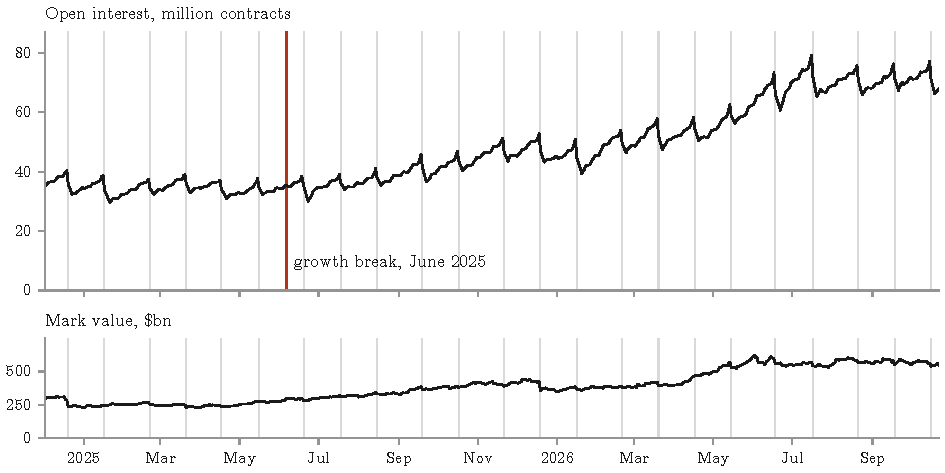
\includegraphics[width=\textwidth]{figures/growth.pdf}
\caption{FLEX open interest (top) and its mark value (bottom) on every activity date
from \PanelStart{} to \PanelEnd{}. Faint vertical lines mark the standard monthly
expiries. The coloured line is the break from a one-break fit to log open interest.}
\label{fig:growth}
\end{figure}

Read off the two ends of the panel (Table~\ref{tab:panel}), open interest grew from
\OIStart{} to \OIEnd{} million contracts and mark value from \ValueStart{} to
\ValueEnd{}. Two single days are a poor guide to growth in this
market, though, because open interest has a monthly sawtooth (Figure~\ref{fig:growth})
and the two ends fall at different points of it. We measure growth in two ways that
do not depend on the day chosen.

The first is a one-break fit. We regress log open interest on calendar time with a
single change of slope, continuous at the break, and choose the break by least squares
over every activity date with at least forty dates on either side. The break falls on
\BreakDate{}. The fitted trend runs at $\PreBreakGrowth$ a year before it and
$\PostBreakGrowth$ a year after. The date is not an artefact of the sawtooth: fitted
to the first activity date after each monthly expiry alone, or to the last date before
each expiry alone, the same model moves the break by at most \BreakShiftDays{} days. We
date the turn on open interest rather than mark value, which also moves with the
prices of the underlyings.

The second is the average over each complete expiry cycle, from the day after one
monthly expiry to the next. Before the break the cycle averages lie between
\OIFlatLow{} and \OIFlatHigh{} million contracts, a mean of \OIFlatLevel{} million, and
they stay inside that band through the cycle ending \FlatBandEnd{}: the fitted break
dates a change of slope, not the first cycle above the old level. The latest complete
cycle, which ended on \OICycleLatestEnd{}, averages \OICycleLatest{}
million, \GrowthMultiple{} times that level. The highest reading on any single date is
\OIPeak{} million, on \OIPeakDate{}.

The fit is descriptive. It dates the turn and says nothing about its cause, and one
break cannot capture the most recent cycles, which have barely grown: the latest cycle
average is $\OIQuarterChange$ on the one a quarter earlier, where the trend fitted after
the break would give $\PostBreakGrowthQuarter$.

\subsection{The expiry cycle}
\label{sec:lifecycle}

The sawtooth in Figure~\ref{fig:growth} is the expiry cycle. Open interest builds
through each month and falls when the standard monthly expiry, the third Friday,
clears. The fall is spread over two reports: an expiring series is still listed on its
expiry date with part of its open interest, and gone on the next activity date. Of the
ten largest one-day falls in the panel, measured against the previous date's level,
\DropsOnExpiry{} land on a monthly expiry or the activity date after it:
\DropsOnExpiryDate{} on the expiry date and \DropsDayAfter{} on the date after. Few would
by chance, since only \ExpiryWindowChanges{} of the \DailyChanges{} day-to-day changes in
the panel, \ExpiryWindowShare{}, span an expiry in this way. The ten falls come from
\DropExpiries{} expiries, and each removes between \DropLow{} and \DropHigh{} of open
interest. On each of those days the series expiring lose more open interest than the market as a whole, between
\ExpiringRatioLow{} and \ExpiringRatioHigh{} times the net fall; the rest of the book
grew on the same days.

\begin{figure}[t]
\centering
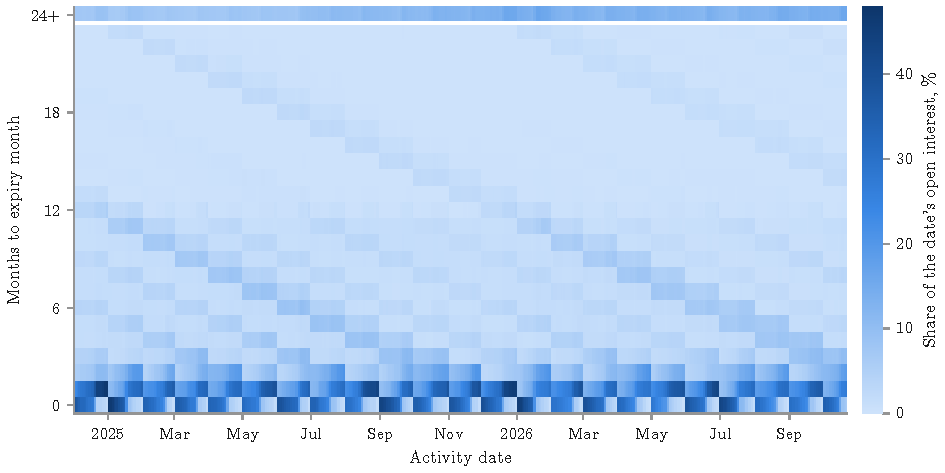
\includegraphics[width=\textwidth]{figures/maturity.pdf}
\caption{Each activity date's open interest by calendar months until its expiry month
(0 is the activity date's own month), as a share of that date's total, on a linear
scale. The top row gathers every expiry \MapHorizonMonths{} or more months ahead:
\BeyondHorizonMean{} of open interest on an average date and \BeyondHorizonShare{} on
the last.}
\label{fig:maturity}
\end{figure}

Figure~\ref{fig:maturity} shows where that open interest sits in maturity. The two
bottom rows, the current month and the next, hold the largest shares, and they alternate
within each month as the third Friday clears the front cohort; the faint diagonal
stripes above them are single cohorts moving towards expiry. On an average date
\WithinSixtyMean{} of open interest expires within sixty days, and the
open-interest-weighted median time to expiry is \MedianDaysMean{} days, between
\MedianDaysLow{} and \MedianDaysHigh{} depending on the date. Roughly half the book
therefore rolls off within two months and is replaced.

Behind that front sits a long-dated tail that has grown faster than the market: open interest more than a year from expiry was
\OverOneYearStart{} of the total on the first date and \OverOneYear{} on the last, and
more than two years out \OverTwoYearsStart{} and \OverTwoYears{}. The sixty-day share
itself ranges from \WithinSixtyLow{} to \WithinSixtyHigh{} over the panel, so the
maturity profile of any one date can sit well away from the typical one.

\subsection{Concentration}

Growth came with breadth. The number of underlyings with FLEX open interest rose from
\UnderlyingsStart{} on the first date to \UnderlyingsEnd{} on the last, and the share
held by the ten largest fell from \TopTenShareStart{} to \TopTenShare{}. On the last
date the five largest are \TopFiveUnderlyings{}; the largest 25 hold
\TopTwentyFiveShare{} of open interest and the largest 100 hold \TopHundredShare{}
(Figure~\ref{fig:concentration}).

\begin{figure}[t]
\centering
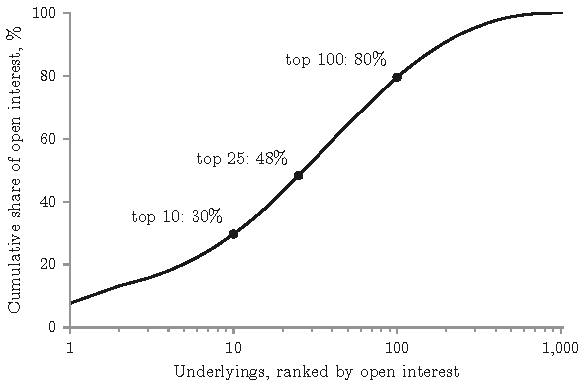
\includegraphics[width=0.62\textwidth]{figures/concentration.pdf}
\caption{Cumulative share of open interest held by the largest underlyings on
\PanelEnd{}, ranked by open interest.}
\label{fig:concentration}
\end{figure}

\section{Two measurement results}

\subsection{Identifying FLEX without the authoritative report}

Listed strikes fall on a standard grid of whole dollars, halves and quarters, which
suggests treating an off-grid strike as FLEX. Table~\ref{tab:confusion} scores that
rule against the report over 486,895 cleared series.

\begin{table}[t]
\centering
\caption{The off-grid heuristic against the authoritative FLEX report.}
\label{tab:confusion}
\begin{tabular}{lrr}
\toprule
& True FLEX & Not FLEX \\
\midrule
Off-grid strike & 4,914 & 2,389 \\
On-grid strike & 9,321 & 470,271 \\
\midrule
\multicolumn{3}{l}{Precision $0.673$ \quad Recall $0.345$ \quad $F_1$ $0.456$} \\
\bottomrule
\end{tabular}
\end{table}

The rule misses 9,321 FLEX series, 65.5\% of the FLEX in that universe, because FLEX is
routinely struck on the grid --- a series such as \texttt{1AAON} at \$99.00 is FLEX at a
round strike and no strike-based test can find it. A third of what the rule flags is
not FLEX at all.

The consequence for anyone tempted by the same reasoning is that a strike-based
identification of FLEX is not merely noisy but severely biased, and the bias is
invisible without the authoritative source.

\subsection{Cleared series are not economic positions}

Open interest is reported per series. Positions span series. Three cases, each found
while building an earlier census, show what conflating them costs.

\paragraph{A butterfly.} One underlying carries call lines of 100k, 200k and 100k
contracts at equally spaced strikes across three consecutive expiries. Read as nine
independent positions this is \$63.8bn of notional. A butterfly cannot be worth more
than its strike spacing times its wing size: \$1.30bn in total, an overstatement of 49
times.

\paragraph{A collar.} SPY at one expiry carries four legs near 37,500 contracts each ---
a synthetic long, a cap, a floor and a buffer floor. The position is roughly \$2.87bn.
Counted leg by leg at strike-based notional it is \$8.02bn.

\paragraph{A strike-based notional.} The same collar's synthetic long call, struck at
\$1.87 against a spot near \$765, carries \$2.9bn of exposure and is recorded by strike
times contracts as \$7m. Deep in-the-money calls used to replicate an underlying are
three orders of magnitude invisible to that measure, while far out-of-the-money legs
are inflated by it.

The errors have opposite signs and do not cancel. The report's mark prices avoid the
valuation half of the problem directly, since they price each series as cleared.

\section{Does hidden inventory predict the visible market?}
\label{sec:predict}

If dealers' listed hedging of FLEX inventory matters, inventory at $T$ should say
something about the underlying once the report can be read. We estimate
\begin{equation}
y_{i,t+1}
= \alpha_i + \delta_t
+ \beta\,\text{flex}_{i,t}
+ \gamma' \text{controls}_{i,t}
+ \varepsilon_{i,t},
\label{eq:pred}
\end{equation}
with the controls and errors of Table~\ref{tab:pred} \citep{cameron2011}. Each report meets
the returns realised from the date it could first be acted on (Section~\ref{sec:panel}),
and a change spanning a date the underlying did not report is dropped. The innovation is
log open interest less its mean over the previous twenty reports. Bars are fetched by the
equity report's tickers, and a bare index symbol names another security or none, so the
\PredIndexUnderlyings{} index underlyings are out. Of the \PredQualifying{} equity names
with at least \PredQualifyingDates{} activity dates, \PredNoBars{} have symbols the
provider does not serve. Adjusted-deliverable roots, option classes renamed with a digit
after a corporate action changed their deliverable (\texttt{GME1}), account for
\PredNoBarsAdjusted{}; share-class spellings such as \texttt{BRKB} for
\PredNoBarsShareClass{}; other tickers, delisted and renamed names among them, for
\PredNoBarsOther{}. That leaves \PredUnderlyingDays{}
underlying-days, \PredUnderlyings{} underlyings and \PredDates{} activity dates.

\begin{table}[t]
\centering
\caption{Hidden inventory at $T$ and the underlying's volatility from $T+1$.}
\label{tab:pred}
\begin{tabular}{llrrrrr}
\toprule
Predictor & Outcome & $10^4\beta$ & $t$ & $10^4\,$MDE80 & Clust.\ $p$ & Perm.\ $p$ \\
\midrule
Inventory innovation & $|r_{t+1}|$ & $-0.37$ & $-0.68$ & 1.53 & 0.50 & 0.45 \\
Inventory change & $|r_{t+1}|$ & $-0.68$ & $-0.64$ & 2.99 & 0.52 & 0.46 \\
Near-dated share change & $|r_{t+1}|$ & $-1.67$ & $-0.44$ & 10.74 & 0.66 & 0.67 \\
Put share & $|r_{t+1}|$ & $+0.56$ & $+0.22$ & 7.19 & 0.83 & 0.61 \\
Inventory innovation & $r_{t+1}^2$ & $+0.06$ & $+0.47$ & 0.34 & 0.64 & 0.71 \\
Placebo: innovation at $T+2$ & $|r_{t+1}|$ & $+1.02$ & $+1.86$ & 1.53 & 0.063 & 0.057 \\
\bottomrule
\end{tabular}
\par\smallskip{\footnotesize Underlying and date fixed effects; standard errors clustered by underlying and by date. Controls: mean absolute return over the previous 5 and 22 sessions, the same day's absolute return, and log dollar volume. 377,332 underlying-days, 1,407 underlyings, 468 activity dates; the placebo row loses the last two dates. Coefficients and MDE80, the effect detectable with 80\% power at the 5\% level, are multiplied by $10^4$, which for $|r|$ is basis points. Clust.\ $p$ uses the clustered errors; Perm.\ $p$ comes from 1,000 re-estimations with the predictor shuffled across underlyings within each date.\par}
\end{table}


Nothing predicts. The innovation's coefficient on next-day absolute return is
$\PredInnovBeta\times10^{-4}$ at $t=\PredInnovT$, and $\PredOpenCloseBeta\times10^{-4}$ at
$t=\PredOpenCloseT$ on the open-to-close return, which leaves out the overnight move,
part of which precedes publication. Mean absolute return over three, five and ten sessions gives
$t=\PredHorizonThreeT$, $\PredHorizonFiveT$ and $\PredHorizonTenT$, and the tenth of
underlying-days with the largest inventory changes $t=\PredDecileT$. Later start dates
move the estimates, not the conclusion (Table~\ref{tab:windows}). The largest genuine
$|t|$ in all of these is \PredMaxAbsT{}.

\begin{table}[t]
\centering
\caption{The main estimate and its placebo with the panel loaded from later dates.}
\label{tab:windows}
\begin{tabular}{lrrrrr}
\toprule
Panel from & Underlying-days & Innovation $\beta\times10^4$ & $t$ & Placebo $\beta\times10^4$ & $t$ \\
\midrule
2024-12-02 & 377,332 & $-0.37$ & $-0.68$ & $+1.02$ & $+1.86$ \\
2025-07-23 & 264,825 & $-0.19$ & $-0.27$ & $+0.98$ & $+1.38$ \\
2025-09-09 & 239,318 & $+0.16$ & $+0.22$ & $+0.93$ & $+1.23$ \\
\bottomrule
\end{tabular}
\par\smallskip{\footnotesize Next-day $|r|$ on the inventory innovation and on its placebo, with the specification of Table~\ref{tab:pred}, rebuilding the panel from each start date. The first row is the full panel.\par}
\end{table}


The permutation test shuffles the predictor across underlyings within each date
(Figure~\ref{fig:placebo}). It treats underlyings as exchangeable within a date, and it
breaks each underlying's own inventory persistence along with any link to its
volatility. For the innovation the draws have a standard deviation of
$\PredNullSd\times10^{-4}$, against a clustered standard error of
$\PredInnovSE\times10^{-4}$; Table~\ref{tab:pred} gives both $p$-values for each row.

\begin{figure}[t]
\centering
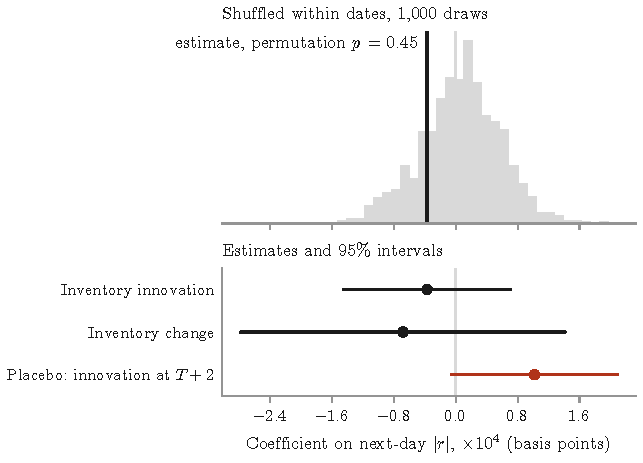
\includegraphics[width=0.68\textwidth]{figures/placebo.pdf}
\caption{Top: the innovation's coefficient on next-day $|r|$, predictor shuffled within
dates. Bottom: estimates and 95\% intervals, same axis; share predictors omitted.}
\label{fig:placebo}
\end{figure}

The placebo is the innovation two activity dates later, dated after its outcome, so it
cannot predict it: $\PredPlaceboBeta\times10^{-4}$ at $t=\PredPlaceboT$, clustered
$p=\PredPlaceboClusterP$, permutation $p=\PredPlaceboPermP$. Whatever association it shows
can only run from the outcome to later inventory, or through something common to both.

The minimum detectable effect at 80\% power is $\PredInnovMDE\times10^{-4}$ per log point
of innovation, \PredMDEShare{} of the mean next-day absolute return. Strike-local,
intraday and option-surface effects are not ruled out.

\section{Limitations}

\begin{enumerate}
\item \textbf{Gross, unsigned inventory.} Open interest does not identify who is long,
and is aggregated across holders. No measure here is a dealer position.
\item \textbf{A short panel.} \PanelMonths{} months, set by how far back OCC's rolling
retention reached when collection began. That is enough to date one turn in growth, and
too short to say whether the levelling of the latest cycles will last.
\item \textbf{One outcome family.} Realised volatility in the underlying, not the option
surface.
\item \textbf{No structure decomposition in the panel.} The measurement section shows
that positions span series; the predictive tests use per-underlying aggregates and
inherit none of that decomposition.
\end{enumerate}

\section{Conclusion}

The FLEX market is publicly reported and larger than its absence from chain data
suggests. A one-break fit dates the start of its growth to \BreakMonth{}. Averaged over
the latest expiry cycle, its open interest is \OICycleLatest{} million contracts,
\GrowthMultiple{} times the level before, though the latest quarter added only
$\OIQuarterChange$, and on the last date it carried \ValueEnd{} of mark value. Much of
it is near expiry, with \WithinSixtyMean{} expiring within sixty days on an average
date, and its monthly sawtooth is that expiry cycle. Beside that front, the share more
than a year from expiry has grown from \OverOneYearStart{} to \OverOneYear{}.

Whether it tells us anything about the visible market is a separate question, and at
the resolution available the answer is no. Per-underlying hidden inventory does not
predict subsequent realised volatility: neither the clustered errors nor, on next-day
volatility, a permutation test finds a predictor, and a placebo dated after its outcome
has a larger $|t|$ than any genuine predictor. An effect of \PredMDEShare{} of the mean daily absolute return per log point
of inventory would have been found four times in five.

Two measurement findings travel further than the setting. A natural strike-based rule
for identifying FLEX recovers a third of it. And cleared series are not economic
positions --- a distinction worth three orders of magnitude in one of the cases here,
with errors that do not cancel.

\section*{Data and code availability}

Every input is free and public. Collection infrastructure, the panel builder, the
tests, and results as they were produced --- including figures later superseded by the
authoritative report --- are available at the project repository.

\begin{thebibliography}{99}

\bibitem[Bollen and Whaley(2004)]{bollen2004}
Bollen, N.~P.~B. and R.~E. Whaley (2004).
Does net buying pressure affect the shape of implied volatility functions?
\emph{Journal of Finance} 59(2), 711--753.

\bibitem[Cameron et al.(2011)]{cameron2011}
Cameron, A.~C., J.~B. Gelbach, and D.~L. Miller (2011).
Robust inference with multiway clustering.
\emph{Journal of Business and Economic Statistics} 29(2), 238--249.

\bibitem[G\^{a}rleanu et al.(2009)]{garleanu2009}
G\^{a}rleanu, N., L.~H. Pedersen, and A.~M. Poteshman (2009).
Demand-based option pricing.
\emph{Review of Financial Studies} 22(10), 4259--4299.

\bibitem[Ni et al.(2005)]{ni2005}
Ni, S.~X., N.~D. Pearson, and A.~M. Poteshman (2005).
Stock price clustering on option expiration dates.
\emph{Journal of Financial Economics} 78(1), 49--87.

\bibitem[Park and Kurucak(2025)]{park2025}
Park, T. and U.~Kurucak (2025).
Growth of income funds and death of volatility.
Working paper, University of Texas at Dallas.

\end{thebibliography}

\end{document}
